\documentclass{amsart}

\usepackage{babel}
\usepackage{textcomp}
\usepackage{mathrsfs}
\usepackage{url}
\usepackage{amstext}
\usepackage{amsthm}
\usepackage{amssymb}
\usepackage{stmaryrd}
\usepackage{float}
\usepackage{pgfplots}
\usepackage{agt}

\begin{document}

\author{Victor Porton}
\email{porton@narod.ru}

\title[Algebraic General Topology]{Algebraic General Topology summary}

\maketitle

In my book~\cite{volume-1-edition1} I introduce some new concepts
generalizing general topology, including \emph{funcoids} and \emph{reloids}.
The book along with supplementary materials (such as a partial draft of the second volume)
is freely available (including the \LaTeX\ source) online.

Before studying funcoids, in my book I consider
co-brouwerian lattices and lattices of filters in particular,
as the theory of funcoids is based on theory of filters.
My book contains probably the best (and most detailed) published overview of properties of filters.

Later I discovered~(\cite{volume-3}) that funcoids and reloids as well as all
kinds of spaces in general topology are a special case of
elements of ordered semigroup actions\footnote{Ordered semigroup actions are first time researched by myself.}. Ordered semigroup actions are a special case of ordered precategory actions, which encompass all things of general topology.

Also I discovered~(\cite{volume-1-edition1} and~\cite{limit}) a definition of a generalization of limit for arbitrary (even discontinuous) functions. This definition has the property that the customary limit or the absence thereof can be restored knowing my generalized limit. Now formulas like \[ \int_a^b f(x)dx - \int_a^b f(x)dx = 0 \] are well defined for an arbitrary function~$f$ (not only for integrable functions). I also started the research of non-differentiable solutions of differential equations.

\section{Conventions}

Because you always can refer to my book, in this short intro I present theorems without proofs.

I denote order on a poset as~$\sqsubseteq$ and corresponding lattice operations as~$\bigsqcup$ and~$\bigsqcap$.
I denote the least and greatest elements (if they exist) of our poset as~$\bot$ and~$\top$ correspondingly.

I call elements~$a$ and~$b$ of a poset \emph{intersecting} and
denote $a\nasymp b$ when there is a non-least~$c$ such that $c\sqsubseteq a\land c\sqsubseteq b$.

For a lattice with the least element we have
\[ a\nasymp b \Leftrightarrow a\sqcap b\ne\bot. \]

\section{Filters}

We will consider \emph{filters} on a set~$\mho$ that is sets~$\mathfrak{F}$ of subsets of~$\mho$ such that
\[ \forall X,Y\in\subsets\mho:
(X,Y\in\mathcal{F} \Leftrightarrow X\cap Y\in\mathcal{F}). \]

Filters are a generalization of sets, allowing to express such things as the infinitely small neighbourhood of zero on the real line: $\setcond{X\in\subsets\mathbb{R}}{\exists\epsilon>0:X\supseteq\left]\epsilon;\epsilon\right[}$.

\begin{defn}
I order the set~$\mathfrak{F}$ of filters (including the improper filter) \emph{reverse} to set-theoretic order, that is
$\mathcal{A} \sqsubseteq \mathcal{B} \Leftrightarrow \mathcal{A} \supseteq \mathcal{B}$
for $\mathcal{A},\mathcal{B}\in\mathfrak{F}$.
\end{defn}

\begin{prop}
This makes the set of filters on a set into a co-brouwerian (and thus distributive) lattice, that is we have
$\mathcal{A} \sqcup \bigsqcap S = \bigsqcap_{\mathcal{X}\in S} (\mathcal{A} \sqcup \mathcal{X})$
for a set~$S$ of filters and a filter~$\mathcal{A}$.
\end{prop}

Wee denote $\uparrow A$ the pricnipal filter corresponding to a set~$A$ that is the filter $\setcond{X\in\subsets\mho}{X\supseteq A}$.

\section{Funcoids}

Let $\mathfrak{F}(A)$, $\mathfrak{F}(B)$ be sets of filters on sets~$A$,~$B$.
They are complete atomistic co-brouwerian lattices.

\begin{defn}
A \emph{funcoid} $A\rightarrow B$ is a quadruple $(A,B,\alpha,\beta)$
where~$\alpha$ and~$\beta$ are functions $\mathfrak{F}(A)\rightarrow \mathfrak{F}(B)$
and $\mathfrak{F}(B)\rightarrow \mathfrak{F}(A)$ correspondingly, such that
$\mathcal{Y} \sqcap \alpha(\mathcal{X}) \ne \bot \Leftrightarrow \mathcal{X} \sqcap \beta(\mathcal{Y}) \ne \bot$
for every $\mathcal{X}\in\mathfrak{F}(A)$, $\mathcal{Y}\in\mathfrak{F}(B)$.
\end{defn}

\begin{defn}
I denote $(A,B,\alpha,\beta)^{-1} = (B,A,\beta,\alpha)$.
\end{defn}

\begin{defn}
I denote $\langle(A,B,\alpha,\beta)\rangle = \alpha$.
\end{defn}

Funcoids generalize such things as:
\begin{itemize}
\item binary relations;
\item proximity spaces;
\item pretopologies;
\item preclosures.
\end{itemize}

For a proximity~$\delta$, define
\[ \mathcal{X}\mathrel{\delta'}\mathcal{Y} \Leftrightarrow \forall X\in\mathcal{X},Y\in\mathcal{Y}: X\mathrel{\delta}Y \]
for all filters~$\mathcal{X}$,~$\mathcal{Y}$.
Then we have a unique funcoid~$f$ such that
\[
\mathcal{X}\mathrel{\delta'}\mathcal{Y} \Leftrightarrow
\mathcal{Y}\sqcap\langle f\rangle\mathcal{X} \ne \bot \Leftrightarrow
\mathcal{X}\sqcap\langle f^{-1}\rangle\mathcal{Y} \ne \bot.
\]

\begin{defn}
$\mathcal{X} \mathrel{[f]} \mathcal{Y} \Leftrightarrow \mathcal{Y}\sqcap\langle f\rangle\mathcal{X} \ne \bot \Leftrightarrow
\mathcal{X}\sqcap\langle f^{-1}\rangle\mathcal{Y} \ne \bot$.
\end{defn}

\begin{prop}
A funcoid~$f: A\rightarrow B$ is uniquely determined by $\langle f\rangle$ and moreover is uniquely
determined by values of the function~$\langle f\rangle$ on principal filters or
by the relation~$[f]$ between principal filters.
\end{prop}

See my book for formulas for \emph{principal funcoids} that is funcoids corresponding to binary relations
and for funcoids corresponding to pretopologies and preclosures (particularly funcoids corresponding to
topological spaces, as topological spaces can be considered as a special case of either pretopologies or preclosures).

There are also several other equivalent ways to define funcoids.

Funcoids are made more interesting than topological spaces by a new operation (missing in traditional general topology),
\emph{composition}, which is defined by the formula
\[ (B,C,\alpha_2,\beta_2)\circ (A,B,\alpha_1,\beta_1) = (A,C,\alpha_2\circ\alpha_1,\beta_1\circ\beta_2). \]

\begin{defn}
$\mathcal{X}\suprel{f}\mathcal{Y} \Leftrightarrow \mathcal{Y}\nasymp\supfun{f}\mathcal{X}$.
\end{defn}

We can define the funcoid~$\uparrow f$ corresponding to a binary relation~$f$ by the formula $\supfun{\uparrow f}\uparrow X=\uparrow\rsupfun{f}X$ for every set~$X$ on its source. (It can be proved that for every~$f$ there exists a unique~$\uparrow f$.) We call funcoids corresponding in this way to binary relations \emph{principal funcoids}.

The following are equivalent definitions of a \emph{complete} funcoid:

??

\section{Reloids}

Reloids are basically just filters on cartesian product~$A\times B$ of two given sets~$A$ and~$B$.

Formally:

\begin{defn}
A \emph{reloid} is a triple $(A,B,F)$ where $A$,~$B$ are sets and $F$ is a filter on~$A\times B$.
\end{defn}

Reloids are a generalization of uniform spaces and of binary relations.

\begin{defn}
Composition $g\circ f$ of reloids can be easily defined as the reloid determined by the filter base
consisting of compositions of binary relations defining these reloids (see the book for an exact formula).
\end{defn}

\begin{prop}
Composition of reloids (and of funcoids) is associative.
\end{prop}

The sets of funcoids and reloids constitute complete atomistic co-brouwerian lattices and these lattices have interesting
properties.

There are interesting relationships between funcoids and reloids, as well as special classes of funcoids and reloids.

\section{Continuity}

A function~$f$ from a space~$\mu$ to a space~$\nu$ is \emph{continuous} iff
$f\circ\mu\sqsubseteq \nu\circ f$. This formula works for continuity, proximal continuity,
uniform continuity, etc., so making all kinds of continuity described by the same formula.

If~$f$ is a principal funcoid or reloid correspondign to a monovalued entirely defined function, then this formula is
equivalent to the following two other formulas:
\[ \mu\sqsubseteq f^{-1}\circ\nu\circ f;\quad
f\circ\mu\circ f^{-1}\sqsubseteq \nu. \]

\section{Spaces as elements of ordered semigroup actions}

\begin{defn}
\emph{Ordered semigroup} (or \emph{posemigroup}) is a set together with binary operation~$\circ$ and binary relation~$\leq$ on it, conforming both to semigroup axioms and partial order axioms and:
\[ x_0\leq x_1\land y_0\leq y_1\Rightarrow y_0\circ x_0\leq y_1\circ x_1. \]
\end{defn}

\begin{defn}
\emph{Ordered precategory} (or \emph{poprecategory}) is
a precategory together with an order on the set of morphisms conforming to the equality:
\[ x_0\leq x_1\land y_0\leq y_1\Rightarrow y_0\circ x_0\leq y_1\circ x_1. \]
\end{defn}

\begin{defn}
\emph{Semiordered precategory action} on~$\mathfrak{A}$ is a precategory action~$\supfun{}$ to the category~$\mathbf{Pos}$ of all partially ordered sets, such that
\begin{enumerate}
\item $a\leq b\Rightarrow\supfun{a}x\leq \supfun{b}x$ for all $a,b\in S$, $x\in\mathfrak{A}$.
\end{enumerate}
I call morphisms of such a precategory as \emph{semi-interspaces}.\footnote{The prefix inter- is supposed to mean that the morphisms may have the source different that the destination.}
\end{defn}

\begin{defn}
\emph{Ordered precategory action} on~$\mathfrak{A}$ is a precategory action~$\supfun{}$ to the category~$\mathbf{Pos}$ of all partially ordered sets, such that
\begin{enumerate}
\item $a\leq b\Rightarrow\supfun{a}x\leq \supfun{b}x$ for all $a,b\in S$, $x\in\mathfrak{A}$;
\item $x\leq y\Rightarrow\supfun{a}x\leq \supfun{a}y$ for all $a\in S$, $x,y\in\mathfrak{A}$.
\end{enumerate}
In other words, an ordered precategory action is a (not necessarily strictly) increasing precategory action (we consider transformations of this action to be ordered pointwise, that is by the product order).

I call morphisms of such a precategory as \emph{interspaces}.
\end{defn}

\begin{defn}
\emph{Curried semiordered semigroup action} on a poset~$\mathfrak{A}$ for an ordered semigroup~$S$ is a function $\supfun{}:S\to(\mathfrak{A}\to\mathfrak{A})$ such that
\begin{enumerate}
\item $\supfun{b\circ a}x = \supfun{b}\supfun{a}x$ for all $a,b\in S$, $x\in\mathfrak{A}$;
$x,y\in\mathfrak{A}$;
\item $a\leq b\Rightarrow\supfun{a}x\leq \supfun{b}x$ for all $a,b\in S$, $x\in\mathfrak{A}$.
\end{enumerate}
I call elements of such an action (that is elements of the corresponding semigroup) \emph{semispaces}.
\end{defn}

\begin{defn}
\emph{Curried ordered semigroup action} on a poset~$\mathfrak{A}$ for an ordered semigroup~$S$ is a function $\supfun{}:S\to(\mathfrak{A}\to\mathfrak{A})$ such that
\begin{enumerate}
\item $\supfun{b\circ a}x = \supfun{b}\supfun{a}x$ for all $a,b\in S$, $x\in\mathfrak{A}$;
$x,y\in\mathfrak{A}$;
\item $a\leq b\Rightarrow\supfun{a}x\leq \supfun{b}x$ for all $a,b\in S$, $x\in\mathfrak{A}$;
\item $x\leq y\Rightarrow\supfun{a}x\leq \supfun{a}y$ for all $a\in S$.
\end{enumerate}
I call elements of such an action \emph{spaces}. (By an element of an action I mean an element of the corresponding semigroup.)
\end{defn}

\begin{rem}
Google search for both ``"ordered semigroup action"'' and ``"action of ordered semigroup"'' and ``"action of an ordered semigroup"'' showed nothing. Was a spell laid onto Earth mathematicians not to find the most important structure in general topology?
\end{rem}

Essentially, an ordered semigroup action is an ordered precategory action with just one object.

The interesting thing here is that every kind of a space
(topological space, uniforms space or reloid, proximity space
of funcoid, metric space) is representable as an element of
an ordered semigroup action. Both spaces and binary relations
(including functions) are interspaces.

All topological properties can be described in terms of
ordered actions of semigroups or more generally ordered actions of precategories.

So, it appears that general topology is nothing other as the
theory of these generalized spaces and interspaces, that is
ordered actions of semigroups or more generally ordered actions of precategories.

\section{Generalized limit}

\subsection{A popular explanation of generalized limit}

For an example, consider some real function~$f$ from $x$-axis to $y$-axis:
\begin{figure}[H]
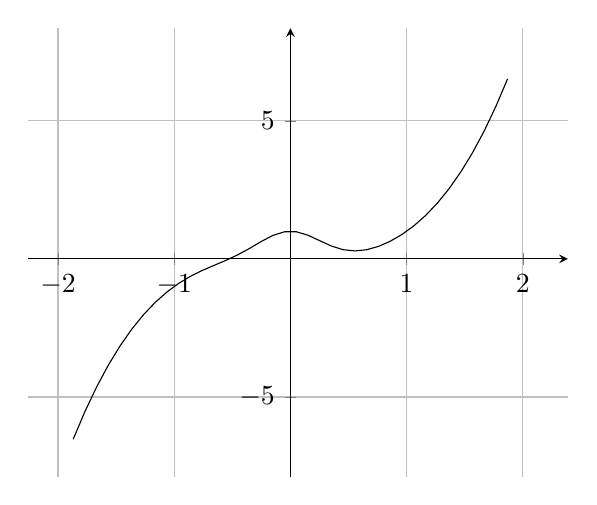
\begin{tikzpicture}
\begin{axis}[grid=both,
          xmax=2,ymax=7,
          axis lines=middle,
          restrict y to domain=-7:7,
          enlargelimits]
\addplot[domain=-5:5,samples=100]{pow(2,-10*x^2)+x^3};
\end{axis}
\end{tikzpicture}
\end{figure}
 
Take it's infinitely small fragment (in our example, an infinitely small interval for~$x$ around zero):
\begin{figure}[H]
\begin{tikzpicture}
\begin{axis}[grid=both,
          xmax=2,ymax=7,
          axis lines=middle,
          restrict y to domain=-7:7,
          enlargelimits]
\addplot[domain=-0.2:0.2,samples=100]{pow(2,-10*x^2)+x^3};
\end{axis}
\end{tikzpicture}
\end{figure}

Next consider that with a value~$y$ replaced with an infinitely small interval like $[y-\epsilon;y+\epsilon]$:
\begin{figure}[H]
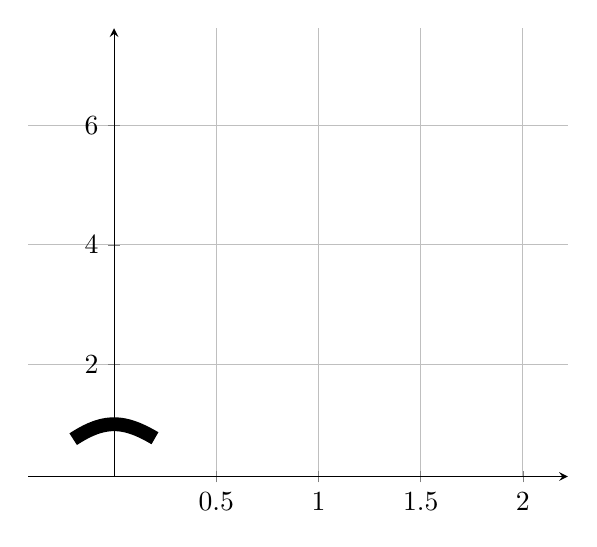
\begin{tikzpicture}
\begin{axis}[grid=both,
          xmax=2,ymax=7,
          axis lines=middle,
          restrict y to domain=-7:7,
          enlargelimits]
\addplot[domain=-0.2:0.2,samples=100,
          line width=5pt]{pow(2,-10*x^2)+x^3};
\end{axis}
\end{tikzpicture}
\end{figure}

Now we have ``an infinitely thin and short strip''. In fact, it is the same as an ``infinitely small rectangle'' (Why? So infinitely small behave, it can be counter-intuitive, but if we consider the above meditations formally, we could get this result):
\begin{figure}[H]
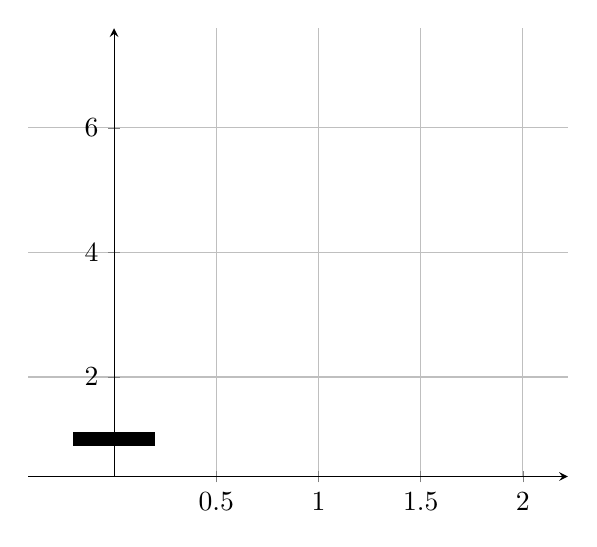
\begin{tikzpicture}
\begin{axis}[grid=both,
          xmax=2,ymax=7,
          axis lines=middle,
          restrict y to domain=-7:7,
          enlargelimits]
\addplot[domain=-0.2:0.2,samples=100,
          line width=5pt]{pow(2,-10)+1};
\end{axis}
\end{tikzpicture}
\end{figure}

This infinitely small rectangle's $y$~position uniquely characterizes the limit of our function (in our example at~$x\to 0$).

If we consider the set of all rectangles we obtain by shifting this rectangle by adding an arbitrary number to~$x$, we get
\begin{figure}[H]
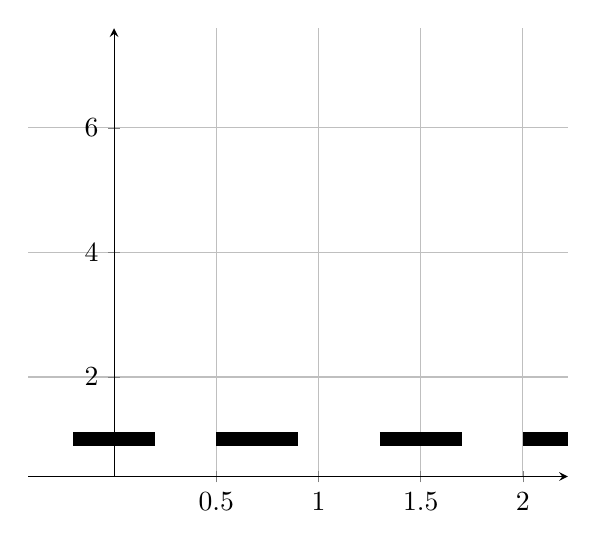
\begin{tikzpicture}
\begin{axis}[grid=both,
          xmax=2,ymax=7,
          axis lines=middle,
          restrict y to domain=-7:7,
          enlargelimits]
\addplot[domain=-0.2:0.2,samples=100,
          line width=5pt]{pow(2,-10)+1};
\addplot[domain=0.5:0.9,samples=100,
          line width=5pt]{pow(2,-10)+1};
\addplot[domain=1.3:1.7,samples=100,
          line width=5pt]{pow(2,-10)+1};
\addplot[domain=2.0:2.4,samples=100,
          line width=5pt]{pow(2,-10)+1};
\addplot[domain=2.7:3.1,samples=100,
          line width=5pt]{pow(2,-10)+1};
\addplot[domain=3.4:3.8,samples=100,
          line width=5pt]{pow(2,-10)+1};
\end{axis}
\end{tikzpicture}
\end{figure}
Such sets one-to-one corresponds to the value of the limit of our function (at $x\to 0$): Knowing such the set, we can calculate the limit (take its arbitrary element and get its so to say $y$-limit point) and knowing the limit value~($y$), we could write down the definition of this set.

So we have a formula for \emph{generalized limit}:
\[ \lim_{x\to a} f(x) =
\{ \nu \circ f|_{\Delta(a)} \circ r \mid r\in G \} \]
where~$G$ is the group of all horizontal shifts of our space~$\mathbb{R}$, $f|_{\Delta(a)}$ is the function~$f$ of which we are taking limit restricted to the infinitely small interval~$\Delta(a)$ around the point~$a$, $\nu\circ{}$~is ``stretching'' our function graph into the infinitely thin ``strip'' by applying a topological operation to it.

What all this (especially ``infinitely small'') means? It is filters and ``funcoids''.

Why we consider all shifts of our infinitely small rectangle? To make the limit not dependent of the point~$a$ to which $x$~tends. Otherwise the limit would depend on the point~$a$.

Note that for discontinuous functions elements of our set (our limit is a set) won't be infinitely small ``rectangles'' (as on the pictures), but would ``touch'' more than just one~$y$ value.

The interesting thing here is that we can apply the above formula to \emph{every} function: for example to a discontinuous function, Dirichlet function, unbounded function, unbounded and discontinuous at every point function, etc. In short, the generalized limit is defined for \emph{every} function. We have a definition of limit for every function, not only a continuous function!

And it works not only for real numbers. It would work for example for any function between two topological vector spaces (a vector space with a topology).

Hurrah! Now we can define derivative and integral of \emph{every} function.

\subsection{Formal}

\fxwarning{The definition with or without~$\uparrow$?}
\fxwarning{``Vertical'' set definitions.}

In~\cite{volume-1-edition1} first defined generalized limit of
a funcoid~$f$ to space~$\nu$ from a group~$G$ of ``translations'':

\begin{defn}
$\lim f=\setcond{\nu\circ f\circ\uparrow r}{r\in G}$.
\end{defn}

Limit of function (or more generally funcoid)~$f$ at filter~$\Delta$ is defined by the formula:

\begin{defn}
$\lim_{\Delta} f=\lim(f|_{\Delta})$.
\end{defn}

For example, limit of~$f:\mu\to\nu$ at point~$a$ is
\[ \lim_{x\to a}f(x) = \lim_{\rsupfun{\mu}\{a\}}f. \]

Generalzed limit can be further generalized to arbitrary spaces
(ordered semigroup actions), but that is not yet thoroughly resaerched yet.

I will call \emph{singularities} the set of generalized limits of the form $\xlim_{\supfun{\mu}\uparrow\{x\}}f$ where $f$~is an entirely defined funcoid and $x$~ranges all points of~$\Ob\mu$.

Let $\operatorname{SNG}(R)$ is the set of singularities for
a set~$R=\Ob\nu$ for some funcoid~$\nu$.

\begin{defn}
\emph{Supersingularities}
\[
\operatorname{SUPER}(R) =
R\cup\operatorname{SNG}(R)\cup
\operatorname{SNG}(\operatorname{SNG}(R))\cup\dots
\]
\end{defn}

We can introduce the structure of a funcoid on supersingularities.

Moreover, we can extend functions on~$\Ob\nu$ to the set
$\operatorname{SUPER}(R)$. It preserves algebraic structures
on~$R$: If $R$~is a group (ring, vector, space, etc.), then $\operatorname{SUPER}(R)$ is a group (ring, vector, space, etc.)

Thus we can consider differential equations
on~$\operatorname{SUPER}(R)$. That is differnetial equations
whose solutions may take infinite values.

It seems this may have applications, e.g. to blackholes.
The author proposes the hypothesis that the center of a blackhole
may contain an infinite quantity of information about its
formation.

\section{Other}

My book~\cite{volume-1-edition1} also considers pointfree generalizations of funcoids,
multidimensional generalizations of funcoids and reloids and other research topics.

My work introduced \emph{many} new conjectures. So I give you a work.

\bibliographystyle{plain}
\bibliography{refs}

\end{document}
